\documentclass[a4paper,11pt]{article}
\usepackage[margin=2cm]{geometry}
\usepackage{graphicx}
\usepackage{color, colortbl}
\usepackage{cite}
\usepackage{url}
\usepackage{float}
\usepackage{arydshln}
\usepackage{pdfpages}
\usepackage{csvsimple}
\usepackage{listings}
\usepackage{algpseudocode}
\usepackage{longtable}
\usepackage{pdflscape}
\usepackage{indentfirst}
\usepackage{mathtools}
\usepackage{amsmath}
\usepackage{amssymb}

\usepackage{tikz}
\usetikzlibrary{matrix,chains,positioning,decorations.pathreplacing,arrows,calc}

% \bibliography{mybib}

\definecolor{Green}{rgb}{0.6,1,0.6}
\definecolor{Amber}{rgb}{1,1,0.4}
\definecolor{Red}{rgb}{1,0.6,0.6}

\def\changemargin#1#2{\list{}{\rightmargin#2\leftmargin#1}\item[]}
\let\endchangemargin=\endlist 

\setlength\parindent{24pt}

\usepackage{fancyhdr}
\pagestyle{fancyplain}
\fancyhf{}
\lhead{\fancyplain{}{M.Sc.\ Individual Project Literature Survey}}
\rhead{\fancyplain{}{\today}}
\cfoot{\fancyplain{}{\thepage}}

\title{Classification of Pipe Weld Images with Deep Neural Networks\\\Large{--- Literature Survey ---}}
\author{Dalyac Alexandre\\
       ad6813@ic.ac.uk\\ \\
       \small{Supervisors: Prof Murray Shanahan and Mr Jack Kelly}\\
       \small{Course: CO541, Imperial College London}
}

\begin{document}

\maketitle

\begin{abstract}

{
Automatic image classification experienced a breakthrough in 2012 with the advent of GPU implementations of deep neural networks. Since then, state-of-the-art has centred around improving these deep neural networks. The following is a literature survey of papers relevant to the task of learning to automatically multi-tag images of pipe welds, from a restrictive number of training cases, and with high-level knowledge of some abstract features. It is therefore divided into 5 sections: foundations of machine learning with neural networks, deep convolutional neural networks (including deep belief networks), multi-tag learning, learning with few training examples, and incorporating knowledge of the structure of the data into the network architecture to optimise learning.\\

In terms of progress, several instances of large-scale neural networks have been trained on a simplifed task: that of detecting clamps in Redbox images. None of them have shown signs of parameter convergence, suggesting that the classification task is particularly challenging. Potential reasons are discussed; the next steps of the project are to test them.
}
\end{abstract}

\clearpage
\tableofcontents

\clearpage
\section{Background}

This project aims to automate the classification of pipe weld images with deep neural networks. After explaining and formalising the problem, we will explain fundamental concepts in machine learning, then go on to explain the architecture of a deep convolutional neural network with restricted linear units, and finally explain how the network is trained with stochastic gradient descent, backpropagation and dropout. The last sections focus on three challenges specific to the pipe weld image classification task: multi-tagging, learning features from a restricted training set, and class imbalance.

\subsection{Defining the Problem}

The problem consists in building a classifier of pipe weld images capable of detecting the presence of multiple characteristics in each image. 

\subsubsection{Explaining the Problem}

Practically speaking, the reason for why this task involves multiple tags per image is because the quality of a pipe weld is assessed not on one, but 17 characteristics, as shown below.

\begin{table}[h]
   \centering
    \begin{tabular}{|l|c|}
    \hline
    Characteristic                 & Penalty Value  \\ \hline
    No Ground Sheet  & ~  5 \\
    No Insertion Depth Markings  & ~ 5 \\
    No Visible Hatch Markings  & ~ 5 \\
    Other  & ~  5 \\
    Photo Does Not Show Enough Of Clamps  & ~ 5 \\
    Photo Does Not Show Enough Of Scrape Zones  & ~ 5 \\
    Fitting Proximity  & ~  15 \\
    Soil Contamination Low Risk  & ~ 15 \\
    Unsuitable Scraping Or Peeling  & ~ 15 \\
    Water Contamination Low Risk  & ~ 15 \\
    Joint Misaligned  & ~  35 \\
    Inadequate Or Incorrect Clamping  & ~ 50 \\
    No Clamp Used  & ~  50 \\
    No Visible Evidence Of Scraping Or Peeling  & ~ 50 \\
    Soil Contamination High Risk  & ~ 50 \\
    Water Contamination High Risk  & ~ 50 \\
    Unsuitable Photo  & ~ 100 \\
    \hline
    \end{tabular}
    \caption {Code Coverage for Request Server}
\end{table} 

At this point, it may help to explain the procedure through which these welds are made, and how pictures of them are taken. The situation is that of fitting two disjoint polyethylene pipes with electrofusion joints \cite{control-point}, in the context of gas or water infrastructure. Since the jointing is done by hand, in an industry affected with alleged "poor quality workmanship", and is most often followed by burial of the pipe under the ground, poor joints occur with relative frequency \cite{control-point}. Since a contamination can cost up to £100,000 \cite{control-point}, there exists a strong case for putting in place protocols to reduce the likelihood of such an event. ControlPoint currently has one in place in which, following the welding of a joint, the on-site worker sends one or more photos, at arm's length, of the completed joint. 

\begin{figure}[h!]
	\centering
	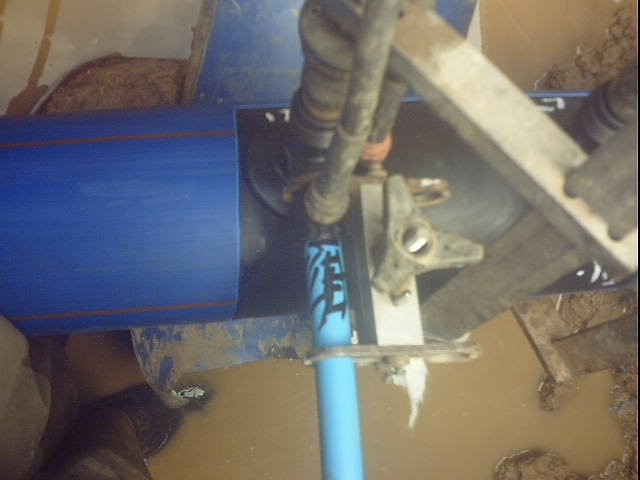
\includegraphics[width=0.3\linewidth]{images/soilcontam2.jpg}
	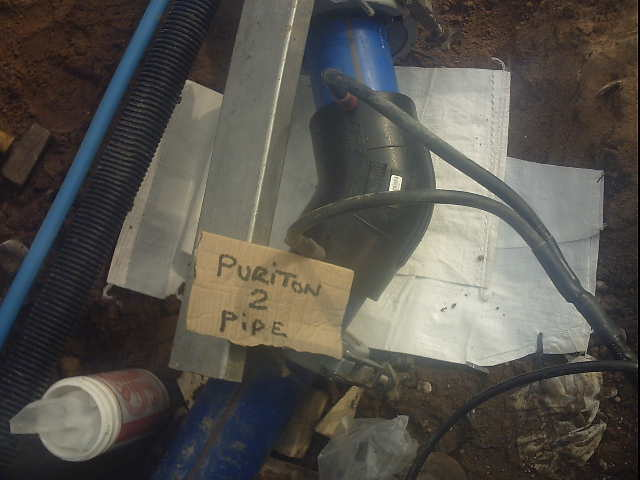
\includegraphics[width=0.3\linewidth]{images/watercontam1.jpg}
	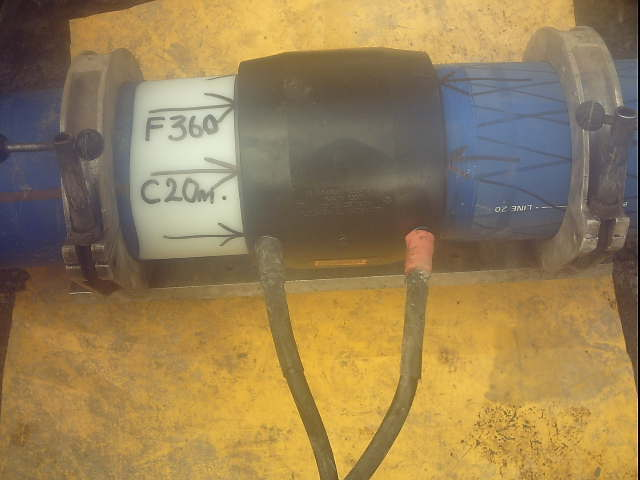
\includegraphics[width=0.3\linewidth]{images/perfect2.jpg}
	\caption{soil contamination risk (left), water contamination risk (centre), no risk (right)}
\end{figure}

These images are then manually inspected at the ControlPoint headquarters and checked for the presence of the adverse characteristics listed above. The joint is accepted and counted as finished if the number of penalty points is sufficiently low (the threshold varies from an installation contractor to the next, but 50 and above is generally considered as unacceptable). Although these characteristics are all outer observations of the pipe fitting, they have shown to be very good indicators of the quality of the weld \cite{control-point}. Manual inspection of the pipes is not only expensive, but also delaying: as images are queued for inspection, so is the completion of a pipe fitting. Contractors are often under tight operational time constraints in order to keep the shutting off of gas or water access to a minimum, so the protocol can be a significant impediment. Automated, immediate classification would therefore bring strong benefits.

\subsubsection{Formalising the problem: Multi-Instance Multi-Label Supervised Learning}

The problem of learning to classify pipe weld images from a labelled dataset is a Multi-Instance Multi-Label (MIML) supervised learning classification problem \cite{MIML}: \\

%\begin{changemargin}{1cm}{1cm}  
\indent Given an instance space $\mathcal{X}$, a set of class labels $\mathcal{Y}$, a dataset $\{(X_{1},Y_{1}),(X_{2},Y_{2}), ..., (X_{n},Y_{n})\}$,\\ 
\indent learn a function $f : 2^{\mathcal{X}} \rightarrow 2^{\mathcal{Y}}$ where\\  
\indent \indent $X_{i} \subseteq \mathcal{X}$ is a set of instances $\{x_{1}^{(i)}, x_{2}^{(i)}, ..., x_{p_{i}}^{(i)}\}$\\   
\indent \indent $Y_{	i} \subseteq \mathcal{Y}$ is the set of classes $\{y_{1}^{(i)}, y_{2}^{(i)}, ..., y_{p_{i}}^{(i)}\}$ such that $x_{j}^{(i)}$ is an instance of class $y_{j}^{(i)}$ 
\indent \indent $p_{i}$ is the number of class instances (i.e.\ labels) present in $X_{i}$.\\
%\end{changemargin}


This differs from the traditional supervised learning classification task, formally given by: \\ 

\indent Given an instance space $\mathcal{X}$, a set of class labels $\mathcal{Y}$, a dataset $\{(x_{1},y_{1}),(x_{2},y_{2}), ..., (x_{n},y_{n})\}$,\\ 
\indent learn a function $f : \mathcal{X} \rightarrow \mathcal{Y}$ where\\  
\indent \indent $x_{i} \in \mathcal{X}$ is an instance \\   
\indent \indent $y_{	i} \in \mathcal{Y}$ is the class of which $x_{i}$ is an instance.\\

In the case of MIML, not only are there multiple instances present in each case, but the number of instances is unknown. MIML has been used in the image classification literature when one wishes to identify all objects which are present in the image \cite{MIML}. Although in this case, the motivation is to look out for a specific set of pipe weld visual characteristics, the problem is actually conceptually the same; the number of identifiable classes is simply lower.

\subsubsection{Supervised Learning}

Learning in the case of classification consists in using the dataset $\mathcal{D}$ to find the hypothesis function $f^{h}$ that best approximates the unknown function $f^{*} : 2^{\mathcal{X}} \rightarrow 2^{\mathcal{Y}}$ which would perfectly classify any subset of the instance space $\mathcal{X}$. Supervised learning arises when $f^{*}(x)$ is known for every instance in the dataset, i.e.\ when the dataset is labelled and of the form $\{(x_{1},f^{*}(x_{1})),(x_{2},f^{*}(x_{2})), ..., (x_{n},f^{*}(x_{n}))\}$. This means that $|\mathcal{D}|$ points of $f^{*}$ are known, and can be used to fit $f^{h}$ to them, using an appropriate cost function $\mathcal{C}$. $\mathcal{D}$ is therefore referred to as the \textit{training set}. 

Formally, supervised learning therefore consists in finding

\begin{equation}
\label{learning: optimisation equation}
  f^{h} = \operatornamewithlimits{argmin}\limits_{\mathcal{F}}\operatorname{\mathcal{C}}(\mathcal{D})
\end{equation}
  
where $\mathcal{F}$ is the chosen target function space in which to search for $f^{h}$ . \\

\subsubsection{Approximation vs Generalisation}

It is important to note that supervised learning does not consist in merely finding the function which best fits the training set - the availability of numerous universal approximating function classes (such as the set of all finite order polynomials) would make this a relatively simple task \cite{univ-approx}. The crux of supervised learning is to find a hypothesis function which fits the training set well \textit{and} would fit well to any subset of the instance space. In other words, approximation and generalisation are the two optimisation criteria for supervised learning, and both need to be incorporated into the cost function.\\

\subsection{Architecture of a Deep Convolutional Neural Network with Rectified Linear Neurons}

Learning a hypothesis function $f^{h}$ comes down to searching a target function space for the function which minimises the cost function. A function space is defined by a parametrised function equation, and a parameter space. Choosing a deep convolutional neural network with rectified linear neurons sets the parametrised function equation. By explaining the architecture of such a neural network, this subsection justifies the chosen function equation. As for the parameter space, it is $\mathbb{R^{P}}$ (where P is the number of parameters in the network); its continuity must be noted as this enables the use of gradient descent as the optimisation algorithm (as is discussed later). \\


\subsubsection{Models of Neurons}

Before we consider the neural network architecture as a whole, let us start with the building block of a neural network: the neuron (mathematically referred to as the \textit{activation function}). Two types of neuron models are used in current state-of-the-art implementations of deep convolutional neural networks: the rectified linear unit and the softmax unit (note that the terms "neuron" and "unit" are used interchangeably). In order to bring out their specific characteristics, we shall first consider two other compatible neuron models: the binary threshold neuron, which is the most intuitive, and the hyperbolic tangent neuron, which is the most analytically appealing. It may also help to know what is being modelled, so a very brief look at a biological neuron shall first be given.

\paragraph{Multipolar Biological Neuron}

\begin{figure}[h!]
	\centering
	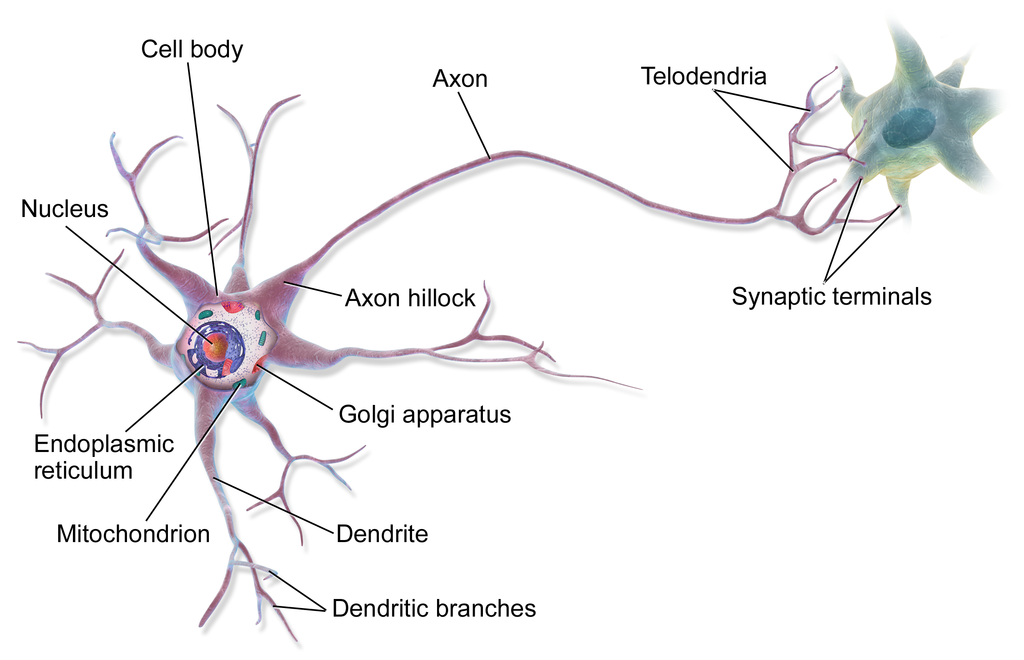
\includegraphics[scale=0.3]{images/Biological_Neuron.png}
	\caption{a multipolar biological neuron}
\end{figure}

A multipolar neuron receives electric charges from neighbouring incoming neurons through its dendritic branches, and sends electric charges to its neighbouring outgoing neurons through its axon. Neurons connect at synapses, which is where the tip of the telodendria of one neuron is in close vicinity of the dendritic branch of another neuron. Because a single axon feeds into all of the telodendria but mutiple dendritic branches feed into the axon hillock, a neuron receives multiple inputs and sends out a single output. Similarly, all of the neuron models below are functions from a multidimensional space to a unidimensional one.\\

\paragraph{Binary Threshold Neuron}
\begin{equation}
y = \begin{cases} 1 & \mbox{if } M <= b + \sum\limits_{i=1}^k x_{i}\cdot w_{i}  \text{ , where } M \text{ is a threshold parameter} \\ 
				  0 & \mbox{otherwise} \end{cases}
\end{equation} \\

Intuitively, $y$ takes a hard decision, just like biological neurons: either a charge is sent, or it isn't. $y$ can be seen as producing spikes, $x_{i}$ as the indicator value of some feature, and $w_[i]$ as a parameter of the function that indicates how important $x_{i}$ is in determining $y$. Although this model is closer than most most to reality, the function is not differentiable, which makes it impossible to use greedy local optimisation learning algorithms - such as gradient descent - which need to compute derivatives involving the activation functions.

\paragraph{Logistic Sigmoid Neuron} 
\begin{equation}
\label{sigmoid neuron}
y = \frac{1}{1 + \exp(-z)} \text{, where } z = \sum\limits_{i=1}^k x_{i}\cdot w_{i}
\end{equation}

Like the binary threshold neuron, the output domain of this neuron is bounded by 0 and 1. But this time, the function is fully differentiable. Moreover, it is nonlinear, which helps to increase performance \cite{DL-book}. To see why, the graph plot below lends itself to the following intuition: if the input x is the amount of evidence for the components of the feature that the neuron detects, and y is the evidence for the feature itself, then the marginal evidence for the feature is decreasing with the amount of evidence for its components (in absolute value terms). 

\begin{figure}[h!]
	\centering
	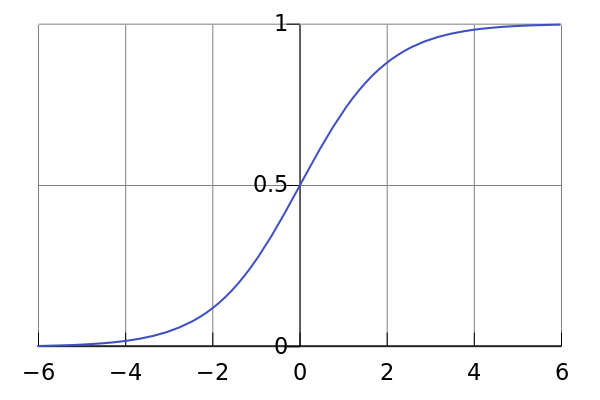
\includegraphics[scale=0.3]{images/sigmoid.png}
	\caption{single-input logistic sigmoid neuron}
\end{figure}

This is like saying that to completely convince y of the total presence or absence of the feature, a lot of evidence is required. However, if there is not much evidence for either case, then y is more lenient. 
A disadvantage of this neuron model is that it is computationally expensive to compute.
                
\paragraph{Rectified Linear Neuron}
\begin{equation}
\label{relu}
y = \max\{0, b + \sum\limits_{i=1}^k x_{i}\cdot w_{i}\}
\end{equation}

As can be seen in the graph plot below, the rectified linear neuron is neither fully differentiable (not at $0$), nor bounded above. Moreover, it only has two slopes, so its derivative with respect to $x_{i}$ can only be one of two values: $0$ or $w_{i}$. Although this may come as a strong downgrade in sophistication compared to the logistic sigmoid neuron, it is so much more efficient to compute (both its value and its partial derivatives) that it enables much larger network implementations\cite{krizhevsky}. Until now, this has more than offset the per-neuron information loss - and saturation risks - of the rectifier versus the sigmoid unit \cite{rectifier}.

\begin{figure}[h!]
	\centering
	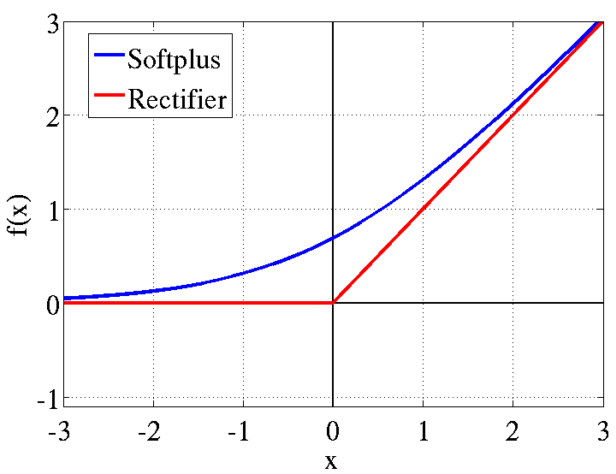
\includegraphics[scale=0.3]{images/rectifier.png}
	\caption{single-input rectified linear neuron}
\end{figure}

\paragraph{Softmax Neuron}
\begin{equation}
\label{}
y_{j} = \frac{\exp(z_{j})}{\sum\limits_{i=1}^k\exp(z_{i})} \text{, where } z_{j} = \sum\limits_{i=1}^k x_{i}\cdot w_{i,j}
\end{equation}

The equation of a softmax neuron needs to be understood in the context of a layer of $k$ such neurons within a neural network: therefore, the notation $y_{j}$ corresponds to the output of the $j^{th}$ softmax neuron, and $w_{i,j}$ corresponds to the weight of $x_{i}$ as in input for the $j^{th}$ softmax neuron. A layer of softmax neurons distinguishes itself from others in that neighbouring neurons interact with each other: as can be seen from the equation, the input vectors of all the softmax neurons $z_{1}, z_{2}, ..., z_{k}$ serve to enforce $\sum\limits_{i=1}^k y_{i} = 1$. In other words, the vector $(y_{1}, y_{2}, ..., y_{k})$ defines a probability mass function. This makes the softmax layer ideal for classification: neuron $j$ can be made to represent the probability that the input is an instance of class $j$. Another attractive aspect of the softmax neuron is that its derivative is quick to compute: it is given by $\frac{dy}{dz} = \frac{y}{1-y}$.


\subsubsection{Feed-Forward Architecture}

A feed-forward neural network is a representation of a function in the form of a directed acyclic graph, so this graph can be interpreted both biologically and mathematically. A node represents a neuron as well as an activation function $f$, an edge represents a synapse as well as the composition of two activation functions $f \circ g$, and an edge weight represents the strength of the connection between two neurons as well as a parameter of $f$. The figure below (taken from \cite{DL-book}) illustrates this.

\begin{figure}[h!]
	\centering
	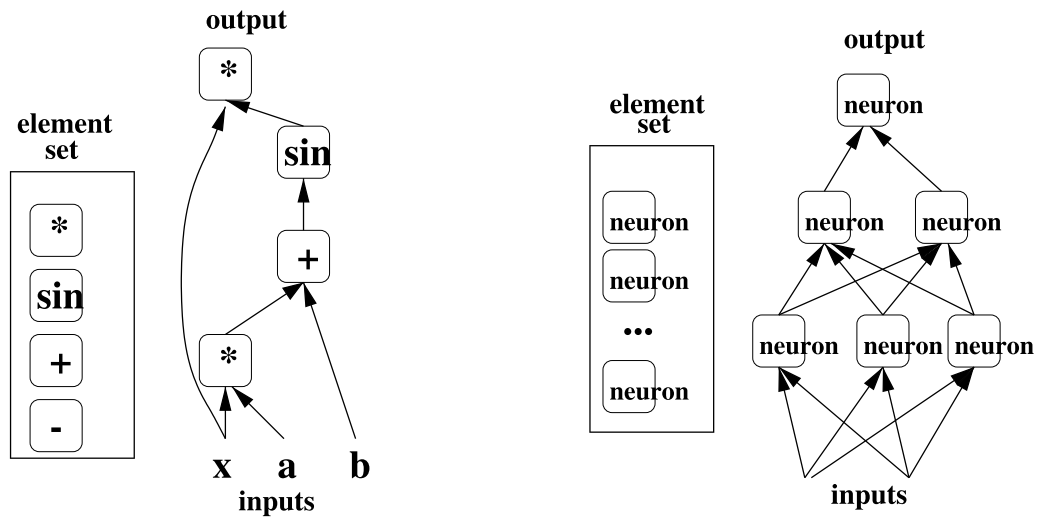
\includegraphics[scale=0.3]{images/NN_math_rep.png}
	\caption{graphical representation of $y = x*sin(a*x+b)$ and of a feed-forward neural network}
\end{figure}

The architecture is feed-forward in the sense that data travels in one direction, from one layer to the other. This defines an input layer (at the bottom) and an output layer (at the top) and enables the representation of a mathematical function.\\

\paragraph{Shallow Feed-Forward Neural Networks: the Perceptron}

A feed-forward neural net is called a perceptron if there exist no layers between the input and output layers. The first neural networks, introduced in the 1960s \cite{DL-book}, were of this kind. This architecture severely reduces the function space: for example, with $g_{1}: x \rightarrow sin(s)$, $g_{2}: x,y \rightarrow x*y$, $g_{3}: x,y \rightarrow x+y$ as activation functions (i.e.\ neurons), it cannot represent $f(x) \rightarrow x*sin(a*x+b)$ mentioned above \cite{DL-book}. This was generalised and proved in \textit{Perceptrons: an Introduction to Computation Geometry} by Minsky and Papert (1969) and lead to a move away from artificial neural networks for machine learning by the academic community throughout the 1970s: the so-called "AI Winter" \cite{Russel & Norvig}.

\paragraph{Deep Feed-Forward Neural Networks: the Multilayer Perceptron}

The official name for a deep neural network is Multilayer Perceptron (MLP), and can be represented by a directed acyclic graph made up of more than two layers (i.e.\ not just an input and an output layer). These other layers are called hidden layers, because the "roles" of the neurons within them are not set from the start, but learned throughout training. When training is successful, each neuron becomes a feature detector. At this point, it is important to note that feature learning is what sets machine learning with MLPs apart from most other machine learning techniques, in which features are specified by the programmer \cite{DL-book}. It is therefore a strong candidate for classification tasks where features are too numerous, complex or abstract to be hand-coded - which is arguably the case with pipe weld images.\\ 

Intuitively, having a hidden layer feed into another hidden layer above enables the learning of complex, abstract features, as a higher hidden layer can learn features which combine, build upon and complexify the features detected in the layer below. The neurons of the output layer can be viewed as using information about features in the input to determine the output value. In the case of classification, where each output neuron corresponds to the probability of membership of a specific class, the neuron can be seen as using information about the most abstract features (i.e.\ those closest to defining the entire object) to determine the probability of a certain class membership. \\

Mathematically, it was proved in 1989 that MLPs are universal approximators \cite{MLP-univ-approx}; hidden layers therefore increase the size of the function space, and solve the initial limitation faced by perceptrons.\\


\paragraph{Deep Convolutional Neural Networks: for translation invariance}

A convolutional neural network uses a specific network topology that is inspired by the biological visual cortex and tailored for computer vision tasks, because it achieves translation invariance of the features. Consider the following image of a geranium: a good feature to classify this image would be the blue flower. This feature appears all across the image; therefore, if the network can learn it, it should then sweep the entire image to look for it. A convolutional layer implements this: it is divided into groups of neurons (called \textit{kernels}), where all of the neurons in a kernel are set to the same parameter values, but are 'wired' to different pixel windows across the image. As a result, one feature can be detected anywhere on the image, and the information of where on the image this feature was detected is contained in the output of the kernel. Below is a representation of LeNet5, a deep convolutional neural network used to classify handwritten characters.

\begin{figure}[h!]
	\centering
	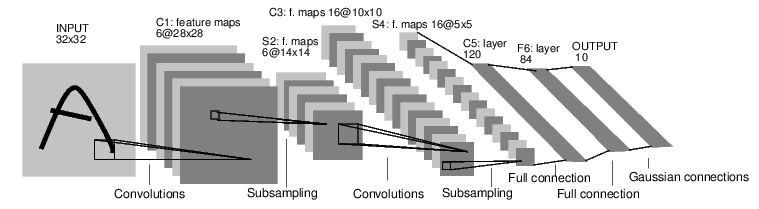
\includegraphics[scale=0.6]{images/lenet5.png}
	\caption{LeNet7 architecture: each square is a kernel}
\end{figure}


\subsection{Training: Backpropagation}

Now that the architecture of a deep CNN has been explained, the question remains of how to train it. Mathematically: now that the function space has been explained, the question remains of how this space is searched. In the case of feed-forward neural networks and supervised learning, this is done with gradient descent, a local (therefore greedy) optimisation algorithm. Gradient descent relies on the partial derivatives of the error (a.k.a\ cost) function with respect to each parameter of the network; the backpropagation algorithm is an implementation of gradient descent which efficiently computes these values.
  
\subsubsection{Compute Error-Weight Partial Derivatives}

Let $t$ be the target output (with classification, this is the label) and let $y = (y_{1}, y_{2}, ..., y_{P})$ be actual value of the output layer on a training case. (Note that classification is assumed here: there are multiple output neurons, one for each class).

The error is given by 
\begin{equation}
E = \mathcal{C}(t-y)
\end{equation}

where $\mathcal{C}$ is the chosen cost function. The error-weight partial derivatives are given by

\begin{equation}
\frac{\partial{E}}{\partial{w_{ij}}} = \frac{\partial{E}}{\partial{y_{i}}} \cdot \frac{\partial{y_{i}}}{\partial{net}} \cdot \frac{\partial{net}}{\partial{w_{ij}}}
\end{equation}

Since in general, a derivative $\frac{\partial{f}}{\partial{x}}$ is numerically obtained by perturbing $x$ and taking the change in $f(x)$, the advantage with this formula is that instead of individually perturbing each weight $w_{ij}$, only the unit outputs $y_{i}$ are perturbed. In a neural network with $k$ fully connected layers and $n$ units per layer, this amounts to $\Theta(k \cdot n)$ unit perturbations instead of $\Theta(k \cdot n^{2})$ weight perturbations (note that the bound on weight perturbations is no longer tight if we drop the assumption of fully connected layers).

\subsubsection{Update Weight Values (with Gradient Descent)}

The learning rule is given by $w_{i,t+1} = w_{i,t+1} + \tau \cdot \frac{\partial{E}}{\partial{w_{i,t}}}$

Visually, this means that weight values move in the direction the will reduce the error quickest, i.e.\ the direction of steepest descent on the error surface is taken. Notice that given the learning rule, gradient descent converges (i.e.\ $w_{i,t+1}$ equals $w_{i,t+1}$) when the partial derivative reaches zero. This corresponds to a local minimum on the error surface. In the figure below, two potential training sessions are illustrated. The minima attained in each cases are not the same. This illustrates a strong shortcoming with backpropagation: parameter values can get stuck in poor local minima.

\begin{figure}[h!]
	\centering
	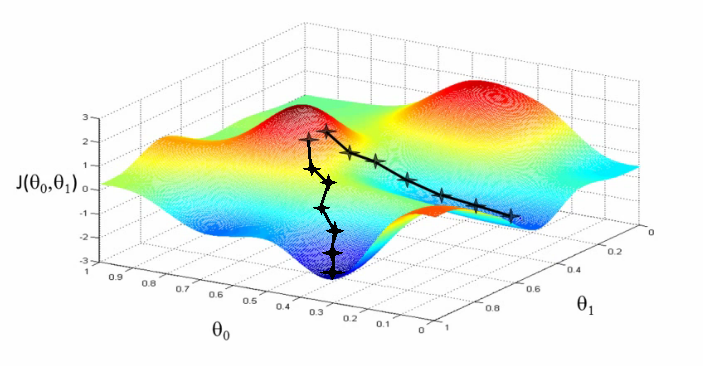
\includegraphics[scale=0.8]{images/local_minima.png}
	\caption{an error surface with poor local minima}
\end{figure}


% \paragraph{cost functions}
% MSE, cross-entropy for softmax

\paragraph{Training, Validation and Test Sets}

As mentioned previously, learning is not a mere approximation problem because the hypothesis function must generalise well to any subset of the instance space. Approximation and generalisation are incorporated into the training of deep neural networks (as well as other models \cite{train&test}) by separating the labelled dataset into a training set, a validation set and a test set. The partial derivatives are computed from the error over the training set, but the function that is learned is the one that minimises the error over the validation set, and its performance is measured on the test set. The distinction between training and validation sets is what prevents the function from overfitting the training data: if the function begins to overfit, the error on the validation set will increase and training will be stopped. The distinction between the test set and the validation set is to obtain a stochastically impartial measure of performance: since the function is chosen to minimise the error over the validation set, there could be some non-negligible overfit to the validation set which can only be reflected by assessing the function's performance on yet another set.

% \paragraph{Dropout}


\subsection{Challenges specific to the Pipe Weld Classification Task}

A number of significant challenges have arisen from this task: multi-tagging, domain change, small dataset size (by deep learning standards) and class imbalance. Before going into them, an overview of the data is given below. \\

\subsubsection{Data Overview}
% \subsubsection{Visual Inspection}
% \subsubsection{Analysis}
% \paragraph{ANOVA}
% \paragraph{t-SNE}


ControlPoint recently upgraded the photographical equipment with which photos are taken (from 'Redbox' equipment to 'Bluebox' equipment), which means that the resolution and finishing of the photos has been altered. There are 113,865 640x480 'RedBox' images. There are 13,790 1280x960 'BlueBox' images. Label frequencies for the Redbox images are given below.

\begin{table}[h]
   \centering
    \begin{tabular}{|l|c|}
    \hline
    Characteristic                 & Count  \\ \hline
    No Ground Sheet  & ~  30,015 \\
    No Insertion Depth Markings  & ~ 17,667 \\
    No Visible Hatch Markings  & ~ 28,155 \\
    Other  & ~  251 \\
    Photo Does Not Show Enough Of Clamps  & ~ 5,059 \\
    Photo Does Not Show Enough Of Scrape Zones  & ~ 21,272 \\
    Fitting Proximity  & ~  1,233 \\
    Soil Contamination Low Risk  & ~ 10 \\
    Unsuitable Scraping Or Peeling  & ~ 2,125 \\
    Water Contamination Low Risk  & ~ 3 \\
    Joint Misaligned  & ~  391 \\
    Inadequate Or Incorrect Clamping  & ~ 1,401 \\
    No Clamp Used  & ~  8,041 \\
    No Visible Evidence Of Scraping Or Peeling  & ~ 25,499 \\
    Soil Contamination High Risk  & ~ 6,541 \\
    Water Contamination High Risk  & ~ 1,927 \\
    Unsuitable Photo  & ~ 2 \\
     \hline
    Perfect (no labels)  & ~ 49,039 \\
    \hline
    \end{tabular}
    \caption {Count of Redbox images with given label}
\end{table} 

\subsubsection{Multi-Tagging}:

As mentioned earlier, training images contain varying numbers of class instances; this uncertainty complexifies the training task.

\subsubsection{Domain Change}:

Domain change can be lethal to machine vision algorithms: for example, a feature learned (at the pixel level) from the 640x480 Redbox images could end up being out of scale for the 1280x960 Bluebox images. However, this simple example is not relevant to a CNN implementation, since the largest networks can only manage 256x256 images, so Bluebox and Redbox images will both be downsized to identical resolutions. However, more worrying is the difference in image sharpness between Redbox and Bluebox images, as can be seen below. It remains to be seen how a CNN could be made to deal with this type of domain change.

\begin{figure}[h!]
	\centering
	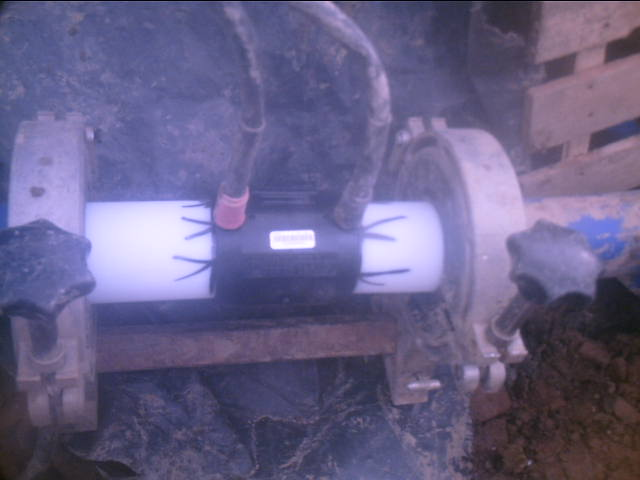
\includegraphics[scale=0.34]{images/perfect3.jpg}
	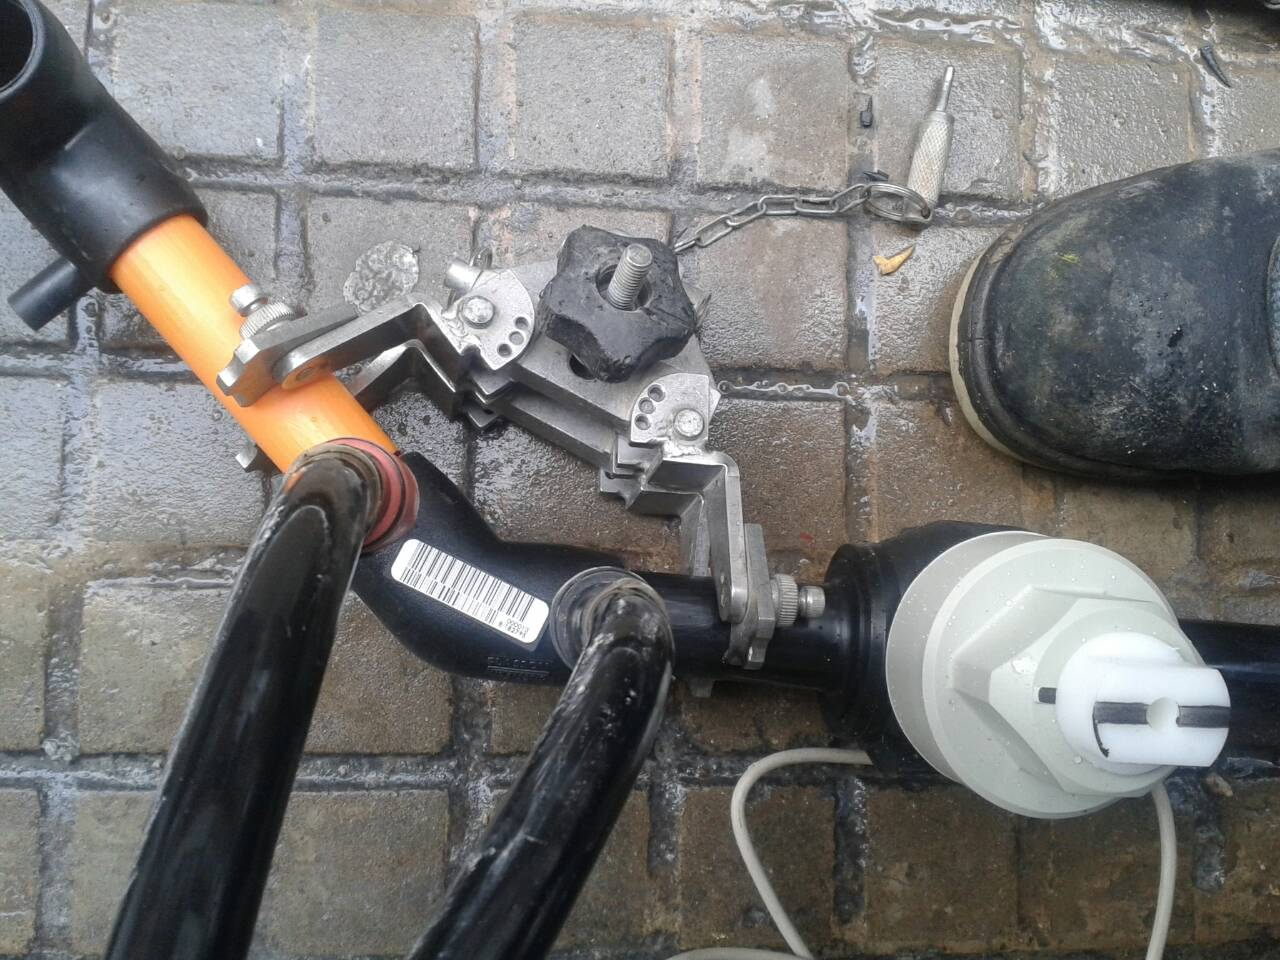
\includegraphics[scale=0.17]{images/niceBluebox_100974.jpg}
	\caption{left: a Redbox photo - right: a Bluebox photo}
\end{figure}

Nevertheless, evidence has been found to suggest that deep neural networks are robust to it: an experiment run by Donahue et al on the \textit{Office} dataset \cite{office}, consisting of images of the same products taken with three different types of photographical equipment (professional studio equipment, digital SLR, webcam) found that their implementation of a deep convolutional neural network produced similar feature representations of two images of the same object even when the two images were taken with different equipment, but that this was not the case when using SURF, the currently best performing set of hand-coded features on the \textit{Office} dataset \cite{surf}. \\

\subsubsection{Small Dataset Size}

Alex Krizhevsky's record-breaking CNN was trained on 1 million images \cite{krizhevsky}. Such a large dataset enabled the training of a 60-million parameter neural network, without leading to overfit. In this case, there are 'only' 127,000, and 43\% of them are images of "perfect" welds, meaning that these are label-less. Training a similarly sized network leads to overfit, but training a smaller network could prevent the network from learning sufficiently abstract and complex features for the task at hand. A solution to consider is that of transfer learning \cite{transfer-learning}, which consists in importing a net which has been pretrained in a similar task with vast amounts of data, and to use it as a feature extractor. This would bring the major advantage that a large network architecture can be used, but the number of free parameters can be reduced to fit the size of the training set by "freezing" backpropagation on the lower layers of the network. Intuitively, it would make sense to freeze the lower (convolutional) layers and to re-train the higher ones, since low-level features (such as edges and corners) are likely to be similar across any object recognition task, but the way in which these features are combined are specific to the objects to detect.

\subsubsection{Class Imbalance}

The dataset suffers from a similar adverse characteristic to that of medical datasets: pathology observations are significantly less frequent that healthy observations. This can make mini-batch training of the network especially difficult. Consider the simple case of training a neural network to learn the following labels: No Clamp Used, Photo Does Not Show Enough Of Clamps, Clamp Detected (this label is not in the list, but can be constructed as the default label). Only 8\% of the Redbox images contain the first label, and only 5\% contain the second label, so if the partial derivatives of the error are computed over a batch of 128 images (as is the case with the best implementations \cite{krizhevsky},\cite{transfer-learning}, \cite{decaf}), one can only expect a handful of them to contain either of the first two labels. Intuively, one may ask: how could I learn to recognise something if I'm hardly ever shown it?\\

One possible solution would be to use a different cost function: the F-measure \cite{f-measure}, which is known to deal with these circumstances. Although the F-measure has been adapted to into a fully differentiable cost function (which is mandatory for gradient descent), there currently exists no generalisation of it for the case of $n \ge 2$
classes. Moreover, one would need to ensure that the range of the error is as large as possible for a softmax activation unit, whose own output range is merely $[0;1]$. \\ \\


\section{Progress}

Following the installation of an open source API for a GPU implementation of a CNN, the pre-processing of the data, and the implementation of data handlers for feeding data into the CUDA code, several instances of large-scale CNNs have been trained on a simplifed task: that of detecting clamps in Redbox images. 

\subsection{Implementation: Cuda-Convnet}

Cuda-Convnet is a GPU implementation of a deep convolutional neural network implemented in CUDA/C++. It was written by Alex Krizhevsky to train the net that set ground-breaking records at the ILSVRC 2012 competition, and subsequently open-sourced. However, parts of his work are missing and his open source repository is not sufficient to reproduce his network. In order to do so, data batching scripts were written for turning raw .jpg images and separate .dat files into pickled python objects each containing 128 stacked jpg values in matrix format with RGB values split across, and a dictionary of labels and metadata for the network. \\

\subsubsection{Test Run}

As mentioned above, several large-scale CNNs have been trained on the clamp detection task using the Redbox data only. The purpose of these models is to set a benchmark for the difficulty of the classification task, by taking several out-of-the-box network configurations: namely, those found on open source projects or detailed in papers \cite{krizhevsky},\cite{transfer-learning}, \cite{decaf}. \\

The classification task is a challenging one: indeed, none of the training sessions have shown any signs of parameter convergence, as the below plot of the validation error over batch iterations can show. 

\begin{figure}[h!]
	\centering
	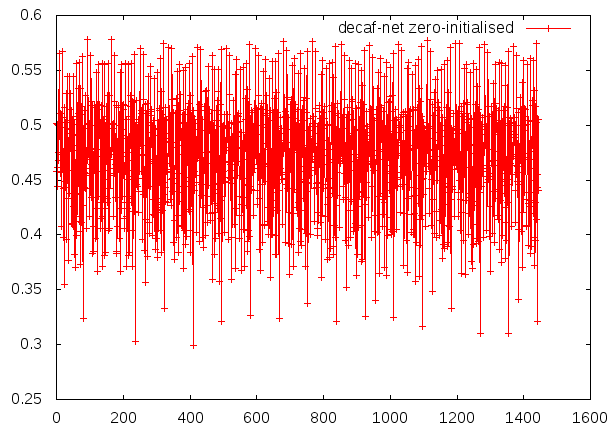
\includegraphics[scale=0.5]{images/logprob.png}
	\caption{validation error rate over batch training iterations}
\end{figure}

There is a wide number of potential explanations for this indirected 'choppiness' in the error rate:
\begin{itemize}
\item The learning rates are too high (the minimum gets 'overshot' even when the direction of partial derivatives is correct)
\item The dropout rate is too high (dropout is a technique which consists in randomly dropping out neurons from the net at every iteration to prevent overfit - but it also means that a different model is tested every time)
\item The number of parameters is too high (the out-of-the-box implementation contains millions of parameters, which is more than than the number of training cases, so collinearities between the parameters cannot even be broken, and most of them are rendered useless)
\item Class imbalance (not enough information about the clampless classes to be able to learn feature for them)
\item Mis-labeled data (at the time of human tagging of these images, tags were left out) \ldots
\end{itemize}
 

The first four explanations are either easy to remedy or interesting to research (particularly the implementation of a wide-ranging, fully differentiable F-Measure, or the import of a pre-trained network). However, if the data is heavily mis-labeled, there may be little that can be done to make this learning task feasible. The next step therefore consists in determining how well-labeled the data is, by way of manual visual inspection on a random (therefore hopefully representative) sample of the training data. \\ \\

\begin{thebibliography}{1}
% Example: \bibitem{One}
% a better way of doing it: a .bib file or something. bit.ly/1kqg2Qe
\bibitem{decaf}
 Donahue, Jeff; Jia, Yangqing; Vinyals, Oriol; Hoffman, Judy; Zhang, Ning; Tzeng, Eric; Darrell, Trevor;
  \emph{DeCAF: A Deep Convolutional Activation Feature for Generic Visual Recognition}\\
  arXiv preprint arXiv:1310.1531, 2013

\bibitem{MIML}
 Zhou, Zhi-Hua; Zhang, Min-Ling;
  \emph{Multi-Instance Multi-Label Learning with Application to Scene Classification}\\
  Advances in Neural Information Processing Systems 19, 
  Proceedings of the Twentieth Annual Conference on Neural Information Processing Systems, 
  Vancouver, British Columbia, Canada, 
  December 4-7, 2006

\bibitem{f-measure}
 Pastor-Pellicer, Joan; Zamora-Martinez, Francisco; Espana-Boquera, Salvador; Castro-Bleda, Maria Jose;
  \emph{F-Measure as the Error Function to Train Neural Networks}\\

\bibitem{control-point}
 Fusion Group - ControlPoint LLP,
 \emph{Company Description}\\
 URL: \url{http://www.fusionprovida.com/companies/control-point}, last accessed 5th June 2014. 
  
\bibitem{univ-approx}
 Barron, Andrew R.,
 \emph{Universal Approximation Bounds for Superpositions of a Sigmoidal Function}\\
 IEEE Transactions on Information Theory, 
 Vol. 39, No. 3
 May 1993

\bibitem{DL-book}
 Bengio, Yoshua;
 \emph{Learning Deep Architectures for AI}\\
 Foundations and Trends in Machine Learning, 
 Vol. 2, No. 1 (2009) 1-127
 2009

\bibitem{Russel & Norvig}
 Russell, Stuart J; Norvig, Peter;
 \emph{Artificial Intelligence: A Modern Approach}\\
 2003

\bibitem{krizhevsky}
 Krizhevsky, Alex; Sutskever, Ilya; Hinton, Geoffrey E.;
 \emph{ImageNet Classification with Deep Convolutional Neural Networks}\\
 2012

\bibitem{rectifier}
 Glorot, Xavier; Bordes, Antoine; Bengio, Yoshua;
 \emph{Deep Sparse Rectifier Neural Networks}\\
 2013

\bibitem{MLP-univ-approx}
 Hornik, Kur; Stinchcombe, Maxwell; White, Halber;
 \emph{Multilayer Feed-Forward Networks are Universal Approximators}\\
 1989

\bibitem{office}
 Saenko, K., Kulis, B., Fritz, M., and Darrell, T.;
 \emph{Adapting visual category models to new domains}\\
 ECCV, 2010

\bibitem{surf}
 Bay, H., Tuytelaars, T., and Gool, L. Van;
 \emph{SURF: Speeded up robust features}\\
 ECCV, 2006

\bibitem{transfer-learning}
 Sermanet, Pierre; Eigen, David; Zhang, Xiang; Mathieu, Michael; Fergus, Rob; LeCun, Yann;
 \emph{OverFeat: Integrated Recognition, Localization and Detection using Convolutional Networks}\\
 arXiv:1312.6229
  
\bibitem{f-measure}
 Joan Pastor-Pellicer, Francisco Zamora-Martínez, Salvador España-Boquera, María José Castro-Bleda;
 \emph{F-Measure as the Error Function to Train Neural Networks}\\
 Advances in Computational Intelligence
 Volume 7902, 2013, pp 376-384
 
\bibitem{cuda-convnet}  
 URL: \url{https://code.google.com/p/cuda-convnet/}, last accessed 6th June 2014.

\end{thebibliography}


\end{document}
